\documentclass{beamer}
%\usetheme{Madrid} % My favorite!
%\usetheme{Boadilla} % Pretty neat, soft color.
%\usetheme{default}
%\usetheme{Warsaw}
\usetheme{Bergen} % This template has nagivation on the left
%\usetheme{Frankfurt} % Similar to the default 
%with an extra region at the top.
%\usecolortheme{seahorse} % Simple and clean template
%\usetheme{Darmstadt} % not so good
% Uncomment the following line if you want %
% page numbers and using Warsaw theme%
\setbeamertemplate{footline}[page number]
\setbeamercovered{transparent}
%\setbeamercovered{invisible}
% To remove the navigation symbols from 
% the bottom of slides%
\setbeamertemplate{navigation symbols}{} 
%
\usepackage{graphics}
%\usepackage{bm}         % For typesetting bold math (not \mathbold)
%\logo{\includegraphics[height=0.6cm]{yourlogo.eps}}
%
\title[Short title of the talk]{How Asymmetry helps Load Balancing \\ \small{\textit{Original Paper by Berthold Vocking}} }
\author{Abhimanyu M A \\ Sumesh T A}
\institute[U of X]
{
Indian Institute of Technology, Kanpur\\
}
\date{\today}
% \today will show current date. 
% Alternatively, you can specify a date.
%
\begin{document}
%
\begin{frame}
\titlepage
\end{frame}
%

\section{Introduction}
\subsection{Classic Problem}
\begin{frame}
\frametitle{Classic Ball Bin Problem}
\begin{block}
{What ?}
Given $n$ balls place them in $n$ bins.
\end{block}
\pause
\begin{block}
{Goal}
Minimizing the number of balls in the largest bin  
\end{block}
\pause
\begin{block}
{Constraints}
\begin{itemize}
\item Balls are indistinguishable
\item Global knowledge of bins are not available
\item Assignment has to be \textit{Online}
\end{itemize}
\end{block}
\end{frame}

\subsection{Classic Algorithm}
\begin{frame}
\frametitle{Classic Randomized Algorithm}
As was seen in such problems Randomization works really well.
\pause
\begin{block}
{Algorithm}
For each ball chose a bin randomly and allocate. 
\end{block}
\pause
\begin{block}
{Expected Load}
$(1+o(1))\frac{ln \; n}{ln \; ln \; n}$ w.h.p
\end{block}
\end{frame}
\subsection{Power of two random choices}
\begin{frame}
\frametitle{Can we do better ?}
Yes we can. \\
\pause
With a little bit more of information \& random bits.\\
\begin{center}
  \textbf{Power of two random choices}
\end{center}
\end{frame}

\begin{frame}
 \frametitle{Power of Two Random Choices}
 Instead of a single bin choose two bins. \\
\pause
\textbf{Not so simple} \\
\pause
\begin{enumerate}
 \item Requires double the number of random bits. \\
 \item Requires Communication. \\
\end{enumerate}
\pause
\begin{block}
{Algorithm}
\begin{enumerate}
 \item Choose $2$ bins randomly, uniformly from set of $n$ bins. 
\item Find bin with lower number of balls. 
\item Add ball to that bin.
\end{enumerate}
\pause
\end{block}
\begin{block}
{Expected Load}
$\frac{ln \, ln \; n}{ln \; 2}  \pm \Theta (1)$ w.h.p \pause \textbf{Exponential Reduction}
\end{block}
\pause
\begin{block}
 {Proof}
We shall be presenting a "simpler" proof, while proving our results.
\end{block}
\end{frame}


\begin{frame}
\frametitle{Even more choices}
What if we had more than $2$, say $d \geq 2$ choices for the bins ?
\begin{center}
 \textbf{It doesn't help much}
\end{center}
\pause
\begin{block}
{Expected Load}
$\frac{ln \, ln \; n}{ln \; d}  \pm \Theta (1)$ w.h.p \pause \textbf{Logarithmic Reduction}
\end{block}
\end{frame}

%\section{Algorithm \& Results}

\begin{frame}
\frametitle{Formalizing a few things}
We can see that any algorithm has to be sequential and online. Now there are three classes of algorithms. Consider a set $[n]=\{0,1, \ldots n-1\}$ bins 
\pause
\begin{block}
{Three Classes}
\begin{enumerate}
\item \textit{Uniform \& Independent} - Each of the $d$ locations of the ball are chosen uniformly and randomly from $[n]$
\item \textit{(Non)Uniform \& Independent} - For $1 \leq i \leq d$ the bin for the $i^{th}$ location is chosen from a probability distribution $D_i$.
\item \textit{(Non)Uniform \& (In)Dependent} - The $d$ locations for the balls are chosen at random from the set $[n]^d$ with a probability distribution $D$.
\end{enumerate}
\end{block}
\begin{block}
{}
This includes all possibilities for Sequential and Online Algorithms. 
\end{block}
\end{frame}

\begin{frame}



\frametitle{Always Go Left Greedy Algorithm}
We can do better with a non-uniform algorithm. \pause \\ 
\begin{center}
\textbf{Surprise !!!}                                                        
\end{center}
\pause
\begin{block}
{Algorithm}
\begin{enumerate}
\item Partition the bin into $d$ groups of \textit{almost} equal size. Each group will have size $\Theta(\frac{n}{d})$
\pause
\item The $i^{th}$ location of the ball is taken uniformly randomly from the $i^{th}$ set of bins only. (See non-uniformity).
\pause
\item Insert ball into the minimum bin among them.
\pause
\item If there are more than one bin with same number of minimum balls, choose the \underline{leftmost} bin.  
\end{enumerate}
\end{block}
\pause
The algorithm seems highly \textit{biased} and \textit{intuitively} we may think it is less efficient, but NO
\pause
\begin{block}
{Expected Load}
$\frac{ln \, ln \; n}{d \; ln \; {\phi_d} }  \pm \Theta (1)$ w.h.p \pause \textbf{Linear Reduction}
\end{block}
 
\end{frame}

\begin{frame}
\frametitle{Fibonacci Constant (Detour)}
We shall take a moment to explain $\phi_d$ which is nothing but the Fibonacci Constant for a Fibonacci Equation of order $d$. 
\begin{block}
{Equation}
\begin{eqnarray}
 F_i  = &  F_{i-1} + F_{i-2} + ... F_{i-d} & \text{ If $i > d$} \nonumber \\
  = &  0 & \text{ Otherwise} \nonumber 
\end{eqnarray}
The constant is nothing but $\phi_d=\lim_{n \to \infty} \frac{F_n}{F_{n-1}}$ \\
The smallest value is $\phi_2 = 1.61803...$ and the largest being $\phi_\infty=2$ \\
$\phi_2 < \phi_3 < \phi_4 < ... < 2$
\end{block}



\end{frame}






%
\begin{frame}
\frametitle{Small Note}
To prove the bound is indeed better we can see that $\phi_d > 2^{\frac{d-1}{d}}$ . Applying it we get
\begin{center}
 \begin{equation}
  \frac{ln \, ln\;d}{d\;ln \; \phi_d} <   \frac{ln \, ln\;d}{d-1\;ln \; 2} <   \frac{ln \, ln\;d}{\;ln \; d} \nonumber
 \end{equation}
\end{center}
\end{frame}
%

\begin{frame}
\frametitle{Theorems}
\begin{theorem}
Suppose that $n$ balls are placed \textit{sequentially} into $n$ bins using the Always-Go-Left Algorithm then the number of balls in the fullest bin is \\
\begin{center}
$\frac{ln \, ln \; n}{d \; ln \; {\phi_d} }  \pm \Theta (1)$ w.h.p
\end{center}
\end{theorem}
Even more importantly
\begin{theorem}
Suppose that $n$ balls are placed \textit{sequentially} into $n$ bins using \textit{any} arbitrary sequential allocation scheme that choose $d$ bins for each ball at random according to an arbitrary probability distribution on $[n]^d$ (Class 3). Then then number of balls in the fullest bin is   \\
\begin{center}
$\frac{ln \, ln \; n}{d \; ln \; {\phi_d} }  - O(1)$ w.h.p
\end{center}
\end{theorem}


\end{frame}

\begin{frame}
\begin{center}
 \textbf{Proof of Upper Bound}
\end{center}

\end{frame}

\begin{frame}
\frametitle{Witness Trees}
\begin{block}
{What}
Think about ``Delay Sequences'' witness trees can be thought of as the tree version of ``delay sequence''. \\
Let $\varepsilon$ be some event, given that $\varepsilon$ has happened it can lead us to infer that few other events $\varepsilon_i$ would have happened (pre-requisites), which in turn would again have other events as pre-requisites hence the tree structure. \\
Even though not found in literature, we found it easy to visualize it 
\end{block}
\begin{example}
Suppose $\varepsilon$ is $i^{th}$ bin has $x$ balls after the $j^{th}$ step. It says that all the $d$ bins chosen during the $j^{th}$ step should have had atleast $x-1$ balls.
\end{example}
\end{frame}

\begin{frame}
\frametitle{What we intend to do}
\begin{enumerate}
\item We intend to use the witness tree to upper bound the probability of a bad event. 
\item An ``activated witness tree'' is a tree that can be constructed for a given event, we shall be looking at the same for the \textit{bad events} 
\item Initially we will be doing a HUGE SIMPLIFICATION we will assume that each ball is included only once in the witness tree, this is as expected wrong but we will be later removing this simplification. 
\item We shall be doing the simple math of 
\begin {center}
 \textbf{Probability of bad event = Number of Witness trees possible $\times$ Probability for the ``activation'' of a witness tree.}
\end {center}


\end{enumerate}


\end{frame}

\begin{frame}
\frametitle{Symmetric Witness Tree}
We shall now see how we can use the witness tree argument to come up with a simpler proof for the ``uniform'' algorithm\\
\begin{block}
{Structure} Each symmetric witness tree of order $L$ is a complete d-ary tree of height $L$ with $d^{L}$ leaf nodes. 
\end{block}
\begin{block}
{Node} Each node represents a ball, (infact more than one node may represent the same ball). The nodes have to be proper , that is a node can be the ancestor of only another node that was inserted before it. Each node represents an event that may or may not happen. 
\end{block}
 

\end{frame}

\begin{frame}
\frametitle{Symmetric Witness Tree - Contd.}

\begin{block}
{Edge Event} Consider an edge $e=(u,v)$ where $v$ is the $i^{th}$ child of $u$. Such an edge exists iff the $i^{th}$ location of $u$'s ball points to the same as one of the locations of $v$'s ball. 
\end{block}
\begin{block}
{Leaf Event} A node is a leaf node if at the time of the insertion of the ball , each of the $d$ locations of the ball points to bins that have atleast $3$ additional balls (balls not represented in the witness tree)
\end{block}
What we can see is that we can give any assignment to the nodes, and find the probability that it satisfies all edge events. 

\end{frame}

\begin{frame}
\frametitle{Construction of a Symmetric Witness Tree}
We shall now prove that given that the maximum load is $L+4$ we shall be able to construct a witness tree of order $L$
\begin{center}
 \textbf{On the black board}
\end{center}

\end{frame}

\begin{frame}
\frametitle{Analyzing the Probability}
\begin{block}
{Possibilities} If we notice, we can give any labeling from $1,..,n$ to any of the nodes. Few of them may not make sense but we can easily upper bound the possibilities. \\
Total number of trees $\leq$ $n^m$ where $m$ is the number of nodes. 
\end{block}
\begin{block}
{Probability of Edge} Probability that $v$ is the $i^{th}$ child of $u$ is at most $\frac{d}{n}$ this is because ball $v$ has $d$ bins to select and each of the bin may be selected with probability $\frac{1}{n}$. \\
Probability of Edge $\leq$ $\left( \frac{d}{n} \right) ^{m-1}$ ( $m-1$ edges) 
\end{block}
\begin{block}
{Probability of Leaf} Each leaf node's $d$ choices have to point to a bin that have additional $3$ balls, since the maximum number of bins with this is $\frac{n}{3}$, this probability can not be greater than $\frac{1}{3}$. Hence for each leaf node the probability is $3^{-d}$ \\
Probability for Leaf Event $\leq$ $3^{-d\cdot q}$ where $q$ is number of leaves. 
\end{block}
\end{frame}


\begin{frame}
\frametitle{Analyzing the Probability}
We can now look at the total probability.
\begin{eqnarray}
 \text{Pr[Witness Tree]} \leq n^m \cdot  \left( \frac{d}{n} \right) ^{m-1} \cdot 3^{-d\cdot q}
\end{eqnarray}
We shall now apply the following easy to see bounds 

\begin{eqnarray}
 m \leq & 2q & \text{Internal nodes is less than number of leaves} \nonumber \\
 2d^2 \leq & 3^d & \text{Basic Algebra} \nonumber \\
 q = & d^L & \text{Property of complete $L$ order $d$-ary tree} \nonumber
\end{eqnarray}

\begin{eqnarray}
 n^m \cdot  \left( \frac{d}{n} \right) ^{m-1} \cdot 3^{-d\cdot q} & \leq & n \cdot d ^{2q} \cdot 3^{-d \cdot q} \\
& \leq & n \cdot 2^{-q} \\
& \leq & n \cdot 2^{-d^L}
\end{eqnarray}

\end{frame}

\begin{frame}
\frametitle{Analyzing the Probability}
We now need to come up with a value for $L$  which gives \\
\begin{center} 
$ n \cdot 2^{-d^L} \leq n^{- \alpha}$ \\
$L \geq log_d \, log_2  \; n + log_d(1+\alpha)$
\end{center}
The given value for $L$ satisfies it. 
\end{frame}


\begin{frame}
\frametitle{Asymmetric Witness Tree}
There is only a slight change in the structure, what we see is asymmetric tree has a large size and larger number of leaves, hence probability decreases. 
\begin{block}
{Structure}
The structure is a ``fibonacci tree'' of order $L$ and $d$-ary fibonacci tree. Please note that the number of leaf nodes of fibonacci tree are bounded by $F_d(d \cdot L+ 1) \geq \phi_d^{d \cdot L-1}$ 
\end{block}

\end{frame}

\begin{frame}
\frametitle{Construction of a Asymmetric Witness Tree}
We shall now prove that given that the maximum load is $L+4$ we shall be able to construct a witness tree of order $L$
\begin{center}
 \textbf{On the black board}
\end{center}
\end{frame}

\begin{frame}
\frametitle{Analyzing the Probability}
\begin{block}
{Possibilities} Total number of trees $\leq$ $n^m$ where $m$ is the number of nodes. 
\end{block}
\begin{block}
{Probability of Edge}The same probability but argued in a slightly different way, if the $i^{th}$ location of $u$ has to point to $v$ it has to be one that is chosen from the $i^{th}$ partition containing $\frac{n}{d}$ bins is $\frac{d}{n}$. \\
Probability of Edge $\leq$ $\left( \frac{d}{n} \right) ^{m-1}$ ( $m-1$ edges) 
\end{block}
\begin{block}
{Probability of Leaf} This again we get the same probability but requires explanation. We now know that there are not more than $\frac{n}{3}$ bins but now we have groups, and we do not know the distribution of the bins, but what we can see is that if we let $\beta_i$ to denote the fraction , the probability is $\prod_{i=1}^{d} \beta_i$, by basic law of maths since sum is preserved it is maximum for equal values. 
Probability for Leaf Event $\leq$ $3^{-d \cdot q}$ where $q$ is number of leaves. 
\end{block}
\end{frame}

\begin{frame}
\frametitle{Analyzing the Probability}
We can now look at the total probability.
\begin{eqnarray}
 \text{Pr[Witness Tree]} \leq n^m \cdot  \left( \frac{d}{n} \right) ^{m-1} \cdot 3^{-d\cdot q}
\end{eqnarray}
We shall apply the bounds we already worked out since they apply here as well,except for number of leaves

\begin{eqnarray}
 n^m \cdot  \left( \frac{d}{n} \right) ^{m-1} \cdot 3^{-d\cdot q} & \leq & n \cdot d ^{2q} \cdot 3^{-d \cdot q} \\
& \leq & n \cdot 2^{-q} \\
\end{eqnarray} 
Now by property of $d$-ary Fibonacci trees
\begin{eqnarray}
 q = \phi^{d \cdot L -1}  
\end{eqnarray}
\end{frame}

\begin{frame}

\frametitle{Analyzing the Probability}
\begin{eqnarray}
 \text{Pr[Witness Tree]} \leq n \cdot 2^{-\phi^{d \cdot L -1} }
\end{eqnarray}
Finding out suitable value for $L$ gives. 
\begin{eqnarray}
L \geq \frac{ln \, \; log_2 \; n + ln \; (1+ \alpha)}{d \cdot ln \; \phi_d} +1 
\end{eqnarray}
Which gives us 
\begin{eqnarray}
L = \frac{ln \, \; log_2 \; n}{d \cdot ln \; \phi_d} +O(1) 
\end{eqnarray}
as the required high probability bound. 
\end{frame}
 
\begin{frame}
 \frametitle{Something we have been avoiding}
Remember we talked about having the same ball multiple number of times, which actually helps us but is WRONG. We will now correct that. \\
We call this procedure 
\begin{center}
 \textbf{Pruning}
\end{center}
\begin{block}
 {Procedure}
We consider $L+4+ \kappa$ balls in the maximum bin and construct a ``Full Witness Tree'' and then ``Prune'' it. 
\end{block}
\begin{center}
 \textbf{Construction \& Pruning on Blackboard}
\end{center}
\end{frame}

\begin{frame}
\frametitle{Analysis of Pruned Witness Tree}
First note that we will be upper bounding the number of nodes by $M=2 \kappa (\alpha +1) log_2 \; n$. \textbf{Why ?}
\begin{block}
{Possibilities} Total number of prunings = $M^{\kappa}$
\end{block}
\begin{block}
{Probability of Edge} $\left( \frac{d}{n} \right) ^{m-1}$ ( $m-1$ edges) 
\end{block}
\begin{block}
{Probability of Leaf} $3^{-d \cdot q}$ where $q$ is number of leaves. 
\end{block}
\begin{block}
{Probability of Pruning} If a vertex is pruned then it means the similar vertex existed before, so let $b$ be the cut off vertex and $b'$ the ball seen before, if you look at the parent on of the edge has to point to one of the $d$ locations pointed by $b$, hence probability $\leq$ $\frac{Md}{n}$ , $M$ is added to consider all such vertices. This has to happen for all $\kappa$ cuts. \\
Probability $\leq$ $\left( \frac{Md}{n}\right)^k$
\end{block}
\end{frame}


\begin{frame}
\frametitle{Analysis of Pruned Witness Tree}
\begin{eqnarray}
 \text{Prob} & \leq & M^\kappa \cdot n^{m+1} \cdot \left( \frac{d}{n} \right)^m \cdot 3^{-d \cdot q} \cdot \left( \frac{Md}{n}\right)^k \\
& \leq& n \cdot d^{2q} \cdot 3 ^{-d.q}  \left( \frac{M^2d}{n}\right)^k \\
& \leq & n \left( \frac{M^2d}{n}\right)^k \; \; \; \; \; \; \; \; \text{                    By $ d^2 \leq 3^d$} \\
& \leq & n \left( \frac{(2 \kappa \cdot (\alpha +1) \cdot log_2 \, n)^2 \cdot d}{n}\right)^\kappa \\
& = & n^{-\kappa +1 + o(1)}
\end{eqnarray}
\end{frame}

\begin{frame}
 \begin{center}
  Lower Bound
 \end{center}
\end{frame}

\begin{frame}
\begin{center}
 We shall now show that for any sequential online assignment of balls to bins with maximum of $d$ local queries the maximum load bin will have on expectation $\frac{ln \, ln \; n}{d \ln \phi_d} - O(1)$ balls w.h.p
\end{center}
\end{frame}

\begin{frame}
\frametitle{Lower Bound Simulation}
The major challenge is to control/understand the possibly dependent choices for the $d$- locations. \\ So instead what we do is we say that  an algorithm $A$ on $n$ bins with dependency relation, it can be simulated by another algorithm $B$ on $dn$ bins where the $i^{th}$ location will be taken from $i^{th}$ set of bins. \\
We also give algorithm $B$ global knowledge \\
\end{frame}

\begin{frame}
 \frametitle{Problem Definition- of $B$}
We define the allocation as a $(m,n_1,n_2,\ldots,n_d)$ where we assign at least $m$ balls to at most $\sum n_i$ bins with the conditions that 
\begin{enumerate}
\item The bins are divided into $d$ disjoint groups $N_1, \ldots N_d$ where $|N_i| \leq n_i$ for $1 \leq i \leq d$
\item Each of the balls is placed into one out of the $d$ bins with probability distribution $D: N_1 \times \ldots \times N_d$.
\item The balls are assigned one after the other. We can only look back. 
\end{enumerate}

\end{frame}

\begin{frame}
\frametitle{What we shall prove}
Let $L^*$ denote the total maximum load in all bins, now we define \textit{aggregated load} $L= \sum_{i=1}^d L_i$ where $L_i$ is the size of the largest bin in the set $N_i$. \\
We shall prove that 
\begin{theorem}
 For any $(n,n,\ldots  n)$ allocation scheme $L= \frac{ln \, ln \; n}{ln \; \phi_d} - O(ln \, ln\; d)$ 
\end{theorem}
This shall prove that. \\
\begin{theorem}
Suppose that $n$ balls are placed \textit{sequentially} into $n$ bins using \textit{any} arbitrary sequential allocation scheme that choose $d$ bins for each ball at random according to an arbitrary probability distribution on $[n]^d$ (Class 3). Then then number of balls in the fullest bin is   \\
\begin{center}
$\frac{ln \, ln \; n}{d \; ln \; {\phi_d} }  - O(1)$ w.h.p
\end{center}
\end{theorem}
\end{frame}

\begin{frame}
\frametitle{Experimental Results}
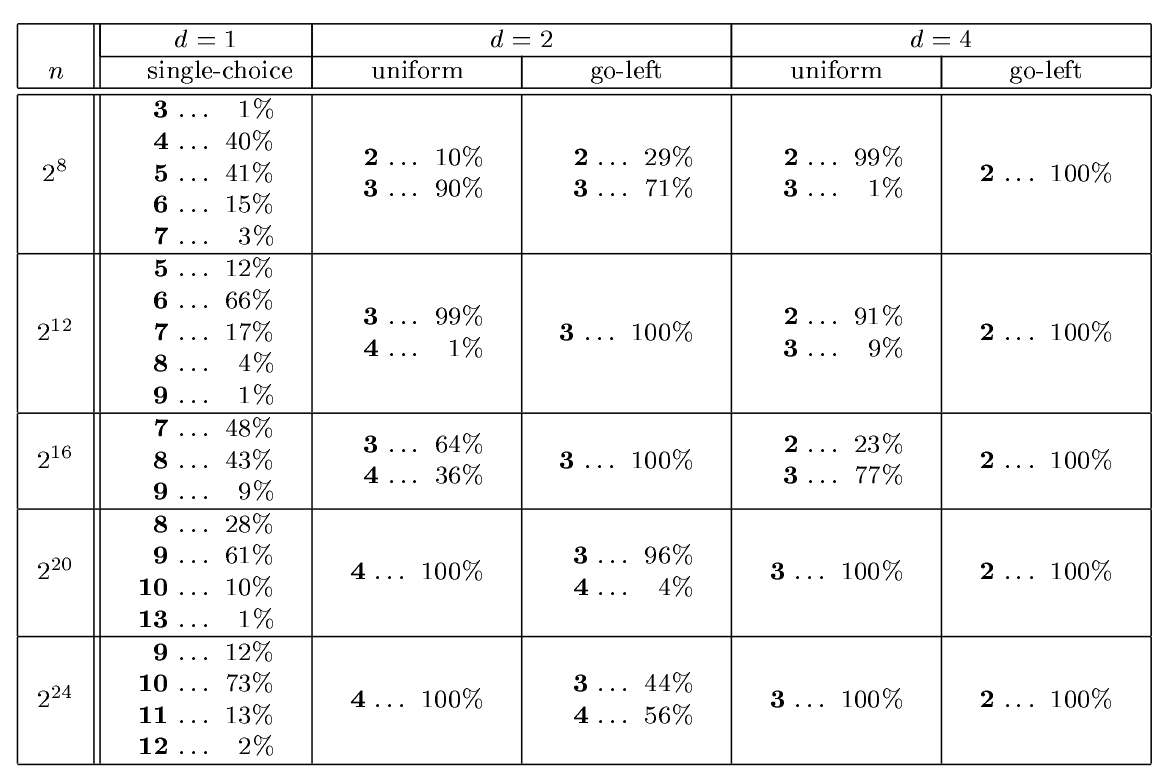
\includegraphics[scale=0.20]{experiment.png}
\end{frame}

\begin{frame}
\frametitle{What we felt}
\begin{enumerate}
\item The algorithm is highly simple, and as we saw has no disadvantages when compared to uniform algorithm. 
 \item The upper bound proof was highly elegant and made simple compared to Adler et al. 
\item The lower bound proof is also very important since it proves that Always Go Left is optimal for all sequential algorithms. 
\item We wonder about the parallel and distributed versions of the algorithm. 
\end{enumerate}

\end{frame}

 
\begin{frame}
\centerline{Questions}
\end{frame}
% End of slides\documentclass{beamer}

\end{document}
